\section{Result 1: the corrected SDE with a learned score at 281 steps}
\label{sec:heun}

With the exact score, Euler--Maruyama leaves a first-order step error in \Sb{}: at $h\approx0.032$, $L=+0.37$ for $P=I$ and $+0.49$ for $\dtwo$.
The Heun-type step of Eq.~\eqref{eq:heun} reduces these to $+0.016$ and $+0.032$ (mean of two seeds).
Here we ask whether this survives a learned score, and in which metrics.

For each metric we ran networks 1--4 with seeds 0 and 1, at four step sizes.
The runs with $h\approx0.032$, $0.016$ and $0.008$ share the Brownian path with the Euler--Maruyama runs of the same network and seed.

\begin{test}[H4, H8: Heun-type \Sb{} with a learned score]
\label{test:heun}
Prediction: at $h\approx0.032$ the median $|L|$ over the eight runs is at most $0.1$ (for $P=I$ and $\dtwo$ also: below the Euler--Maruyama median at $h\approx0.032$ and $0.016$).
\emph{Supported in all four metrics:} the medians are $0.056$ ($P=I$), $0.083$ ($\dtwo$), $0.054$ ($\optc{1.25}$) and $0.073$ ($\optc{5}$), against $0.42$--$0.55$ for Euler--Maruyama on the same path (Table~\ref{tab:heun}, Fig.~\ref{fig:heun}).
\end{test}

\begin{table}[t]
\caption{Corrected SDE \Sb{} with a learned score: median $|L|$ over 8 runs (networks 1--4 $\times$ seeds 0, 1), Heun-type integrator [Eq.~\eqref{eq:heun}] and Euler--Maruyama (EM) on the same Brownian path. $\infty$: at least half of the runs non-finite. $n_{\rm nf}$: non-finite Heun runs; $n_{\rm o}$: Heun runs with at least one outlier.}
\label{tab:heun}
\begin{ruledtabular}
\begin{tabular}{lcccc}
 & $K=140$ & $281$ & $562$ & $1124$ \\
 & $h\approx0.064$ & $0.032$ & $0.016$ & $0.008$ \\
\hline
$P=I$ Heun & $\infty$ & 0.056 & 0.040 & 0.038 \\
\quad EM & $\infty$ & 0.416 & 0.246 & 0.140 \\
\quad $n_{\rm nf}$, $n_{\rm o}$ & 7, 8 & 0, 1 & 0, 0 & 0, 0 \\
$\dtwo$ Heun & $\infty$ & 0.083 & 0.059 & 0.047 \\
\quad EM & $\infty$ & 0.543 & 0.333 & 0.184 \\
\quad $n_{\rm nf}$, $n_{\rm o}$ & 4, 4 & 0, 1 & 0, 1 & 0, 0 \\
$\optc{1.25}$ Heun & 0.153 & 0.054 & 0.036 & 0.035 \\
\quad EM & $\infty$ & 0.445 & 0.257 & 0.144 \\
\quad $n_{\rm nf}$, $n_{\rm o}$ & 3, 3 & 0, 1 & 0, 0 & 0, 0 \\
$\optc{5}$ Heun & 0.207 & 0.073 & 0.035 & 0.027 \\
\quad EM & 0.685 & 0.552 & 0.342 & 0.189 \\
\quad $n_{\rm nf}$, $n_{\rm o}$ & 0, 0 & 0, 0 & 0, 0 & 0, 0 \\
\end{tabular}
\end{ruledtabular}
\end{table}


\begin{observation}[outliers and one broken run at 281 steps]
\label{obs:heun-outliers}
At $h\approx0.032$, 29 of the 32 runs have no outlier and three have one each.
One of these three ($P=I$, network 2, seed 0) is broken: its single outlier gives $|L|=101$.
At $h\approx0.016$ and $0.008$ the medians are $0.027$--$0.059$, and only one run has an outlier (one).
\end{observation}

\begin{observation}[140 steps are not enough]
\label{obs:heun-140}
At $h\approx0.064$ ($K=140$) the Heun-type sampler gives non-finite values in 7 of 8 runs for $P=I$, 4 of 8 for $\dtwo$ and 3 of 8 for $\optc{1.25}$.
For $\optc{5}$ all runs are finite, with $|L|=0.19$--$0.22$.
Euler--Maruyama at the same step is worse in every metric.
This grid is not strictly coupled to the others (App.~\ref{app:methods}).
\end{observation}

The cost of a Heun-type step is two score evaluations, so 281 Heun-type steps cost as much as 562 Euler--Maruyama steps.
At that cost Euler--Maruyama reaches only $|L|=0.25$--$0.34$ (Table~\ref{tab:heun}).
The learned score adds about $0.04$ to $|L|$ (the Heun-type medians at $h\approx0.008$ are $0.027$--$0.047$, while the exact-score Heun values are $\leq0.006$).
This matches the learned-minus-exact shift of \Sb{} at the finest step, $+0.04$.
At 281 steps the step error and the score error are therefore of the same order.
In contrast to the probability-flow ODE (Sec.~\ref{sec:metric}), the metric hardly matters here: the four medians at $h\approx0.032$ lie within $0.054$--$0.083$.

\begin{figure*}[t]
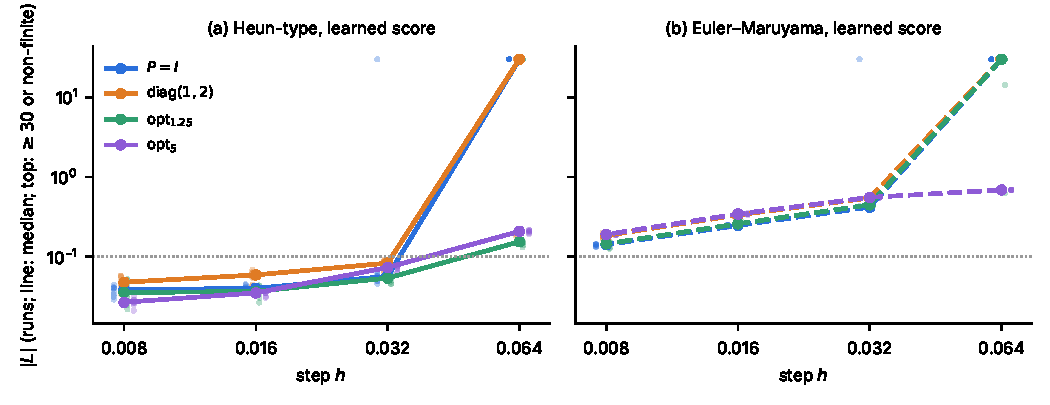
\includegraphics[width=\textwidth]{figures/fig1_heun}
\caption{Corrected SDE \Sb{} with a learned score, four metrics, networks 1--4 $\times$ seeds 0, 1.
(a)~Heun-type integrator, Eq.~\eqref{eq:heun}; (b)~Euler--Maruyama on the same Brownian path ($h\leq0.032$).
Lines: median $|L|$ over the eight runs; dots: runs.
Values of 30 or more, and non-finite values, are drawn at 30.
Dotted: $|L|=0.1$.}
\label{fig:heun}
\end{figure*}
